% Title: glps_renderer figure
% Creator: GL2PS 1.3.8, (C) 1999-2012 C. Geuzaine
% For: Octave
% CreationDate: Mon May 22 01:42:52 2017
\setlength{\unitlength}{1pt}
\begin{picture}(0,0)
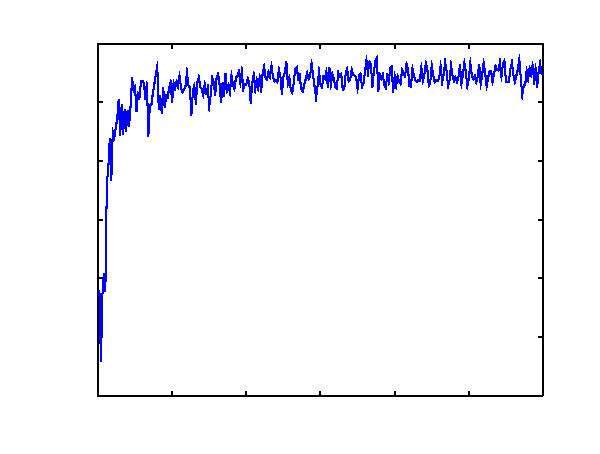
\includegraphics{q11-inc}
\end{picture}%
\begin{picture}(288,218)(0,0)
\fontsize{10}{0}
\selectfont\put(47.0044,22.9956){\makebox(0,0)[t]{\textcolor[rgb]{0,0,0}{{0}}}}
\fontsize{10}{0}
\selectfont\put(82.6104,22.9956){\makebox(0,0)[t]{\textcolor[rgb]{0,0,0}{{50}}}}
\fontsize{10}{0}
\selectfont\put(118.216,22.9956){\makebox(0,0)[t]{\textcolor[rgb]{0,0,0}{{100}}}}
\fontsize{10}{0}
\selectfont\put(153.822,22.9956){\makebox(0,0)[t]{\textcolor[rgb]{0,0,0}{{150}}}}
\fontsize{10}{0}
\selectfont\put(189.428,22.9956){\makebox(0,0)[t]{\textcolor[rgb]{0,0,0}{{200}}}}
\fontsize{10}{0}
\selectfont\put(225.034,22.9956){\makebox(0,0)[t]{\textcolor[rgb]{0,0,0}{{250}}}}
\fontsize{10}{0}
\selectfont\put(260.64,22.9956){\makebox(0,0)[t]{\textcolor[rgb]{0,0,0}{{300}}}}
\fontsize{10}{0}
\selectfont\put(42.0132,27.9961){\makebox(0,0)[r]{\textcolor[rgb]{0,0,0}{{0.15}}}}
\fontsize{10}{0}
\selectfont\put(42.0132,56.1631){\makebox(0,0)[r]{\textcolor[rgb]{0,0,0}{{0.2}}}}
\fontsize{10}{0}
\selectfont\put(42.0132,84.3306){\makebox(0,0)[r]{\textcolor[rgb]{0,0,0}{{0.25}}}}
\fontsize{10}{0}
\selectfont\put(42.0132,112.498){\makebox(0,0)[r]{\textcolor[rgb]{0,0,0}{{0.3}}}}
\fontsize{10}{0}
\selectfont\put(42.0132,140.666){\makebox(0,0)[r]{\textcolor[rgb]{0,0,0}{{0.35}}}}
\fontsize{10}{0}
\selectfont\put(42.0132,168.833){\makebox(0,0)[r]{\textcolor[rgb]{0,0,0}{{0.4}}}}
\fontsize{10}{0}
\selectfont\put(42.0132,197){\makebox(0,0)[r]{\textcolor[rgb]{0,0,0}{{0.45}}}}
\fontsize{10}{0}
\selectfont\put(153.822,11.9956){\makebox(0,0)[t]{\textcolor[rgb]{0,0,0}{{t}}}}
\fontsize{10}{0}
\selectfont\put(17.0132,112.498){\rotatebox{90}{\makebox(0,0)[b]{\textcolor[rgb]{0,0,0}{{$\epsilon_t$}}}}}
\fontsize{10}{0}
\selectfont\put(153.822,207){\makebox(0,0)[b]{\textcolor[rgb]{0,0,0}{{Result of Question 11}}}}
\end{picture}
